\documentclass[landscape]{standalone}
\usepackage{tikz}
\usepackage{intcalc}

\usetikzlibrary{backgrounds,through, intersections, decorations.text, decorations.pathreplacing, calc}
\begin{document}
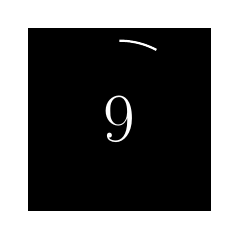
\begin{tikzpicture} [background rectangle/.style={fill=black},show background rectangle]
\def\framesPerSecond{25}
\def\seconds{10}
\def\currentFrame{27};
\def\circleArg{\intcalcMod{\currentFrame}{\framesPerSecond}}
\def\countOfNumber{\intcalcDiv{\intcalcSub{\currentFrame}{\circleArg}}{\framesPerSecond}}
\def\numberToShow{\intcalcSub{\seconds}{\countOfNumber}}
\def\colourA{white}
\def\colourB{black}
\def\modCountOfNumber{\intcalcMod{\countOfNumber}{2}}
\def\colourArcA{\ifnum \modCountOfNumber>0\colourA \else \colourB \fi}
\def\colourArcB{\ifnum \modCountOfNumber>0\colourB \else \colourA \fi}
\def\angle{\intcalcDiv{\intcalcMul{360}{\circleArg}}{\framesPerSecond}}

\node[white, align=center] at (0,0) {\Huge \numberToShow};

%\node[white, align=center] at (0,0) {\Huge \numberToShow~\countOfNumber~\angle~\modCountOfNumber};

\draw [\colourB, thick,domain=0:360] plot ({sin(\x)}, {cos(\x)});

\ifnum \modCountOfNumber>0
\ifnum \angle>0 \draw [\colourA, thick,domain=0:\angle] plot ({sin(\x)}, {cos(\x)});\fi
\else
\ifnum \angle<360 \draw [\colourA,thick,domain=\angle:360] plot ({sin(\x)}, {cos(\x)});\fi
\fi
%\ifnum \angle<360\draw [\colourArcB,thick,domain=\angle:360] plot ({-sin(\x)}, {cos(\x)});\fi
\end{tikzpicture}
\end{document}
